\documentclass{article}

\usepackage[margin=.75in]{geometry}
\usepackage{amsmath}
\usepackage{amssymb}
\usepackage[shortlabels]{enumitem}
\usepackage{pgfplots}
\usepackage{circuitikz}
\usepackage{float}

\author{Damien Prieur}
\title{Final Part 1\\ ECES 511}
\date{}

\begin{document}

\maketitle

\section*{Problem 1}
Determine the convolution of the two signals $p(t)$ and $g(t)$ below.
You can either plot or write down the equation for your answer.
Show all your work and clearly indicate your answer.
\begin{figure}[h!]
\centering
\begin{tikzpicture}[>=stealth]
    \begin{axis}[
        xmin=-.5,xmax=4.5,
        ymin=-.5,ymax=2,
        axis x line=middle,
        axis y line=middle,
        axis line style=->,
        xlabel={$t$},
        ylabel={$p(t)$},
        width=0.45\textwidth,
        height=0.25\textwidth,
        ]
        \addplot[no marks,black,-] expression[domain=0:1,samples=20]{1};
        \addplot[no marks,black,-]coordinates {(1,0)(1,1)};
    \end{axis}
\end{tikzpicture}
\centering
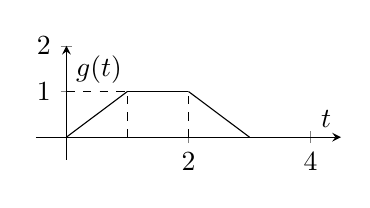
\begin{tikzpicture}[>=stealth]
    \begin{axis}[
        xmin=-.5,xmax=4.5,
        ymin=-.5,ymax=2,
        axis x line=middle,
        axis y line=middle,
        axis line style=->,
        xlabel={$t$},
        ylabel={$g(t)$},
        width=0.45\textwidth,
        height=0.25\textwidth,
        ]
        \addplot[no marks,black, dashed]coordinates {(0,1)(1,1)};
        \addplot[no marks,black,-]coordinates {(0,0)(1,1)};
        \addplot[no marks,black, dashed]coordinates {(1,0)(1,1)};
        \addplot[no marks,black,-]coordinates {(1,1)(2,1)};
        \addplot[no marks,black, dashed]coordinates {(2,0)(2,1)};
        \addplot[no marks,black,-]coordinates {(2,1)(3,0)};
    \end{axis}
\end{tikzpicture}
\end{figure}
We have
$$
y(t) = \int_{0}^{t} g(\tau)p(t-\tau) d\tau
$$
$$
g(t)
=
\begin{cases}
    t       & 0 \leq t \leq 1 \\
    1       & 1 \le  t \leq 2 \\
    -(t-3)  & 2 \le  t \leq 3 \\
    0   & otherwise
\end{cases}
\quad
p(t)
=
\begin{cases}
    1   & 0 \leq t \leq 1 \\
    0   & otherwise
\end{cases}
$$
$$
y(t) = \int_{0}^{t} g(t-\tau)u(\tau) d\tau
=
\begin{cases}
    \int_{0}^{t} \tau d\tau & 0 \leq t \leq 1 \\
    \int_{t-1}^{1} \tau d\tau + \int_{1}^{t} p(t-\tau) d\tau  & 1 \leq t \leq 2 \\
    \int_{t-1}^{2} p(t-\tau) d\tau + \int_{2}^{t} -(\tau -3) p(t-\tau)d\tau  & 2 \leq t \leq 3 \\
    \int_{t-1}^{3} -(\tau-3)p(t-\tau) d\tau & 3 \leq t \leq 4 \\
    0   & otherwise
\end{cases}
$$
$$y(t) =
\begin{cases}
    \frac{ t^2}{2}          & 0 \leq t \leq 1 \\
    \frac{-t^2}{2} + 2t - 1 & 1 \leq t \leq 2 \\
    \frac{-t^2}{2} + 2t - 1 & 2 \le  t \leq 3 \\
    \frac{ t^2}{2} - 4t + 8 & 3 \le  t \leq 4 \\
    0   & otherwise
\end{cases}
$$
\begin{figure}[h!]
\centering
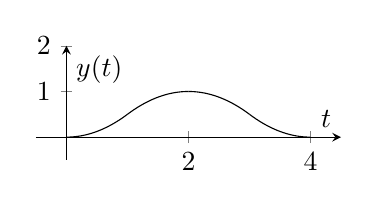
\begin{tikzpicture}[>=stealth]
    \begin{axis}[
        xmin=-.5,xmax=4.5,
        ymin=-.5,ymax=2,
        axis x line=middle,
        axis y line=middle,
        axis line style=->,
        xlabel={$t$},
        ylabel={$y(t)$},
        width=.45\textwidth,
        height=0.25\textwidth,
        ]
        \addplot[no marks,black,-] expression[domain=0:1,samples=30]{x*x/2};
        \addplot[no marks,black,-] expression[domain=1:2,samples=30]{-x*x/2 + 2*x -1};
        \addplot[no marks,black,-] expression[domain=2:3,samples=30]{-x*x/2 + 2*x -1};
        \addplot[no marks,black,-] expression[domain=3:4,samples=30]{x*x/2 - 4*x +8};
    \end{axis}
\end{tikzpicture}
\end{figure}


\newpage
\section*{Problem 2}
Let $v_1=\begin{bmatrix} 1 \\ 3 \\ 5 \end{bmatrix}$,$v_2=\begin{bmatrix} 2 \\ 5 \\ 9 \end{bmatrix}$,$v_2=\begin{bmatrix} -3 \\ 9 \\ 3 \end{bmatrix}$,
\begin{enumerate}[1)]
\item Determine if $\{v_1,v_2,v_3\}$ is linearly independent?
\newline
We can check for independence by performing Gaussian elimination of the matrix comprised of $[v_1 \quad v_2 \quad v_3]$
$$
A =
\begin{bmatrix}
1 & 2 & -3 \\
3 & 5 & 9  \\
5 & 9 & 3
\end{bmatrix}
$$
$$
\begin{bmatrix}
1 & 2 & -3 \\
3 & 5 & 9  \\
5 & 9 & 3
\end{bmatrix}
\implies
\begin{bmatrix}
1 & 2  & -3  \\
0 & -1 & -18 \\
0 & -1 & -12
\end{bmatrix}
\implies
\begin{bmatrix}
1 & 2  & -3  \\
0 & -1 & -18 \\
0 & 0  & -6
\end{bmatrix}
$$
Since we have reduced this to an upper triangular matrix each column is linearly independent from each other.
This implies that the rank of the matrix is $3$.
\item If it is linearly independent find $a$, $b$, $c$ where $av_1 + bv_2 + cv_3 = 0$.
If not, find the relations among $v_1,v_2,v_3$.
\newline
Since all the columns are linearly independent and the rank matches the dimensions of the matrix the null space of $A$ only contains the zero vector.
$$
\begin{bmatrix}a\\b\\c\end{bmatrix}
=
\begin{bmatrix}0\\0\\0\end{bmatrix}
$$
\end{enumerate}

\newpage
\section*{Problem 3}
Given 5 equations:
\begin{align*}
 2a + b &= 20 \\
 6a + b &= 18 \\
20a + b &= 10 \\
30a + b &=  6 \\
40a + b &=  2 \\
\end{align*}
\begin{enumerate}[a)]
\item Find the closest solution $\{a,b\}$ to the five equations.
{\color{blue} Use MATLAB to confirm how "close" it is.}
\newline
If we rewrite the equations into matrix form $Ax=b$
$$
A=
\begin{bmatrix}
2 & 1 \\
6 & 1 \\
20 & 1 \\
30 & 1 \\
40 & 1 \\
\end{bmatrix}
\qquad
x =
\begin{bmatrix} a \\ b \end{bmatrix}
\qquad
b =
\begin{bmatrix}
20 \\
18 \\
10 \\
6  \\
2  \\
\end{bmatrix}
$$
We can solve this equation by performing the pseudoinverse and modifying our original equation with $A^TAx=A^Tb \implies x = (A^TA)^{-1}A^Tb$
\newline
First we compute $A^TA$
$$
A^TA
=
\begin{bmatrix}
2 & 6 & 20 & 30 & 40 \\
1 & 1 & 1 & 1 & 1 \\
\end{bmatrix}
\begin{bmatrix}
2  & 1 \\
6  & 1 \\
20 & 1 \\
30 & 1 \\
40 & 1 \\
\end{bmatrix}
=
\begin{bmatrix}
2940  & 98 \\
98  & 5 \\
\end{bmatrix}
$$
Now we can find the inverse of $A^TA$
$$(A^TA)^{-1}
=
\frac{1}{det(A^TA)}
adj(A^TA)
=
\frac{1}{5096}
\begin{bmatrix}
5 & -98 \\
-98 & 2940 \\
\end{bmatrix}
$$
$$
x = (A^TA)^{-1}A^Tb
=
\frac{1}{5096}
\begin{bmatrix}
5 & -98 \\
-98 & 2940 \\
\end{bmatrix}
\begin{bmatrix}
2 & 6 & 20 & 30 & 40 \\
1 & 1 & 1 & 1 & 1 \\
\end{bmatrix}
\begin{bmatrix}
20 \\
18 \\
10 \\
6  \\
2  \\
\end{bmatrix}
=
\frac{1}{5096}
\begin{bmatrix}
5 & -98 \\
-98 & 2940 \\
\end{bmatrix}
\begin{bmatrix}
608 \\
56
\end{bmatrix}
=
\frac{1}{5096}
\begin{bmatrix}
-2448 \\
105056
\end{bmatrix}
$$
$$
\begin{bmatrix}
a\\
b
\end{bmatrix}
=
\begin{bmatrix}
-0.480377 \\
20.615385
\end{bmatrix}
$$
My error using squared error $(Ax-b)^T(Ax-b)$ was $1.6075$ while matlab's solution using $pinv(A)*x$ was also $1.6075$ and also came to the same numerical solution.


\item Is there any geometric meaning for $\{a,b\}$?
\newline
Each equation can be thought of as a line in the plane and our solution is the point that minimizes the squared error for all equations.
\end{enumerate}

\newpage
\section*{Problem 4}
Using the transfer function $\frac{Y(s)}{R(s)} = \frac{6}{(s+2)(s+3)}$.
\newline
Note this transfer function has no zero/pole cancellation and is a minimal polynomial.
\begin{enumerate}[1)]
\item Convert from Transfer function to Differential equation then to the State equations.
\newline
\item Confirm by converting directly from the Transfer function to the State equation.
{\color{blue} Use MATLAB to confirm.}
\newline
\item Calculate the impulse response of the system.
\newline
\end{enumerate}

\newpage
\section*{Problem 5}
Use the Cayley Hamilton Theorem to find $A^{-1}$ where $A = \begin{bmatrix} 0 & 1 \\ -2 & 3 \end{bmatrix}$.
Validate your answer with $AA^{-1}$.
\newline

\newpage
\section*{Problem 6}
Given the following system with initial conditions:
\begin{align*}
\frac{dx}{dt} &= \begin{bmatrix} -2 & 0 \\ 0 & -4 \end{bmatrix} x(t) + \begin{bmatrix} 4 \\ -1 \end{bmatrix} r(t) \\
y(t) &= \begin{bmatrix} 1 & 3 \end{bmatrix} x(t) \\
x(0) &= \begin{bmatrix} 4 \\ 5 \end{bmatrix} \\
\end{align*}
\begin{enumerate}[a)]
\item Find the state trasition matrix $\varphi (t) = e^{At}$.
{\color{blue} Use MATLAB to confirm}
\newline

\item Find the transfer function $\frac{Y(s)}{R(s)}$ (factor all polynomials).
\newline
\item Find the total solution for the state vector $x(t)$ if the input $r(t) = 2 u(t)$ where $u(t) = unit step function$.
{\color{blue} Use MATLAB to confirm}
\newline
\hspace*{10mm} Clearly identify the \textbf{zero input part} of the solution
\newline
\hspace*{10mm} Clearly identify the \textbf{zero state part} of the solution
\newline
\hspace*{10mm} Then combine into a final result
\newline
Show the results in both the time domain and Laplace domain.
\textbf{Hint:} It is easier to solve if you work in the Laplace domain then convert to the time domain.
\end{enumerate}
\end{document}
